\documentclass[../TDO1-O2.tex]{subfiles}%

\begin{document}
\section[s]"2"{Réfractomètre de \textsc{Pulrich}}
\enonce{%
	\noindent
	\begin{isd}[lefthand ratio=.70]
		Un réfractomètre de \textsc{Pulrich} est constitué d'un bloc de verre de
		section
		rectangulaire d'indice $N$ connu, sur lequel on a déposé une goutte de
		liquide d'indice $n$ inconnu ($n < N$). On observe un faisceau de rayons
		parallèles à la limite réfraction/réflexion totale et on mesure en sortie
		l'angle $\alpha$ dans ce cas.
		\tcblower
		\begin{center}
			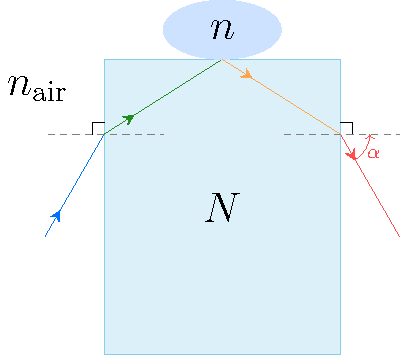
\includegraphics[width=\linewidth]{pulrich_plain}
			\label{fig:pulrich_plain}
		\end{center}
		\vspace{-15pt}
	\end{isd}
	\vspace{-30pt}
}%

\QR{%
	Établir l'expression de $n$ en fonction de $N$ et $\alpha$.
}{%
	\noindent
	\begin{minipage}[t]{.68\linewidth}
		$\DS \sin(i_{\rm lim, N\rightarrow n}) = \frac{n}{N}$ d'une part.
		D'autre part, $N\sin(\theta) = \sin\alpha$, mais on a aussi $\theta =
			\pi/2 - i_{\rm lim}$~: on a donc $\sin\theta = \cos i_{\rm lim} = \DS
			\sqrt{1- \left(\frac{n}{N}\right)^2}$. Ainsi, $\DS\sin^2\alpha = N^2
			\left( 1 - \frac{n^2}{N^2} \right)$~; autrement dit,
		\begin{equation*}
			\boxed{n = \sqrt{N^2 - \sin^2\alpha}}
			\quad\text{avec}\quad
			\left\{
			\begin{array}{rcl}
				N      & = & \num{1.622} \\
				\alpha & = & \ang{60;;}
			\end{array}
			\right.
		\end{equation*}
	\end{minipage}
	\hfill
	\noindent
	\begin{minipage}[t]{.3\linewidth}
		\vspace{0pt}
		\begin{center}
			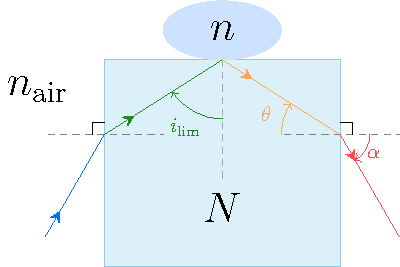
\includegraphics[width=\linewidth]{pulrich}
			\label{fig:pulrich}
		\end{center}
	\end{minipage}
}%

\QR{%
	Application numérique~: calculer $n$ sachant que $N = \num{1.626}$ et
	$\alpha = \ang{60;00;}$.
}{%
	Application numérique~:
	\[\boxed{n = \num{1.376}}\]
}%

\end{document}
